\chapter{Análisis}

\section{Análisis de requisitos}

Todo software se desarrolla para cubrir una necesidad, por lo que en este apartado vamos a describir los requisitos que se estiman necesarios para cubrir los objetivos propuestos.

\subsection{Descripción de los actores}

Los actores implicados serán dos: el \textbf{desarrollador} y el \textbf{usuario}.

\bigskip
El \textbf{desarrollador} será el encargado de solucionar los problemas de visualización de los datos en el portal, además de portar el desarrollo actual del portal a un entorno de desarrollo continuo. También asumirá la administración del portal ya que este tipo de rol está muy integrado con las labores de despliegue en el desarrollo continuo.

\bigskip
El \textbf{usuario} de la aplicación será cualquier persona que tenga interés por conocer datos internos de la \textbf{Universidad de Granada} fácilmente. El usuario no pertenece a ningún público objetivo concreto, por lo que no se tiene que considerar que tenga una experiencia previa en navegador por sitios web.

\bigskip
Los dos tipos de actores descritos son la generalización de todo los tipos de personas que usarían el portal, sin embargo, podríamos hacer un análisis más extenso si nos basáramos en una metodología orientada al usuario como \textbf{persona}. Una persona sería la representación de usuarios que comparten objetivos y a los que se espera comportamientos similares. Un par de ejemplos:

\newpage
\begin{itemize}
	\item Alguien de la propia \textbf{Universidad de Granada} y de otra universidad que accedan al portal, ambos encajarían dentro del actor \textbf{usuario}, sin embargo eso no quiere decir que el objetivo de ambos sea el mismo, los usuarios de la propia universidad pueden querer consultar datos únicamente y los de otra universidad puede que estén más interesados en ver la estructura de las páginas del portal.
	\item Alguien que quiera hacer una despliegue de la aplicación, puede que no quiere hacerlo para una universidad sino para un ayuntamiento, volvemos a estar en el mismo caso, ambos entrarían en el tipo de actor \textbf{desarrollador}, pero sus intenciones e interés son muy distintos entre sí.
\end{itemize}

\subsection{Requisitos funcionales}

Los requisitos funcionales son las características que tiene que implementar el sistema para cubrir todas las necesidades de los distintos usuarios.

\bigskip
Al usuario lo único que le interesa es ver una página web estática con la información que desea 
consultar, para ello el desarrollador deberá hacer que sea posible que se generen siempre las tablas con los elementos de información. 

\bigskip
Por otra parte, el desarrollador quiere integrar el sistema en un desarrollo continuo, por lo que añadirá tests unitarios, test de cobertura, integración continua, despliegue automático y provisionamiento con tal fin.

\begin{itemize}
  \item \textbf{RF-1.} Administración portal:
    \begin{itemize}
    \item \textbf{RF-1.1.} Automatizar inicio del servidor del portal.
    \end{itemize}
\end{itemize}

\begin{itemize}
  \item \textbf{RF-2.} Acceso información:
    \begin{itemize}
    \item \textbf{RF-2.1.} Consultar información de \textit{Administración}.
    \item \textbf{RF-2.1.} Consultar información de \textit{Docencia}.
    \item \textbf{RF-2.1.} Consultar información de \textit{Gestión e Investigación}.
    \item \textbf{RF-2.1.} Consultar información de \textit{Normativa Legal}.
    \end{itemize}
\end{itemize}

\begin{itemize}
  \item \textbf{RF-3.} Pruebas de software:
  \begin{itemize}
    \item \textbf{RF-3.1.} Realizar tests unitarios.
    \item \textbf{RF-3.2.} Realizar test de cobertura.
    \item \textbf{RF-3.2.} Usar integración continua.
    \end{itemize}
\end{itemize}

\begin{itemize}
  \item \textbf{RF-4.} Configuración automática:
  \begin{itemize}
    \item \textbf{RF-4.1.} Usar despliegue automático.
    \item \textbf{RF-4.2.} Usar provisionamiento.
    \end{itemize}
\end{itemize}

\subsection{Requisitos no funcionales}

Los requisitos no funcionales son las características propias del desarrollo, pero que no tienen que estar relacionadas con su funcionalidad.

\begin{itemize}
  \item \textbf{RN-1.} Toda la programación del portal se hará en {\tt Node.js} y los módulos que se usen deben ser instalables a través de su gestor de paquetes {\tt NPM}.
  \item \textbf{RN-2.} El portal se iniciará y se detendrá mediante scripts lanzados con {\tt NPM}.
  \item \textbf{RN-3.} Para iniciar la ejecución del portal es necesario que reciba el puerto de escucha del servidor y la dirección de acceso.
  \item \textbf{RN-4.} Todos los módulos se ejecutarán desde scripts lanzamos con {\tt NPM}.
  \item \textbf{RN-5.} Los tests unitarios se realizarán en base a comportamientos esperados y valores de estados.
  recibidos como contestación a las peticiones que se realicen al portal.
  \item \textbf{RN-6.} Los tests unitarios tienen que recibir las páginas del portal para ejecutarse.
  \item \textbf{RN-7.} El test de cobertura tiene que tener una automatización integrable con los tests unitarios. 
  \item \textbf{RN-8.} La integración continua se ejecutará automáticamente con cada cambio que se haga en la programación del portal.
  \item \textbf{RN-9.} El despliegue automático se realizará mediante conexiones {\tt SSH}.
  \item \textbf{RN-10.} Tanto para el despliegue automático como para el provisionamiento es necesario indicar el usuario que lo realiza y el destino en el que se realiza.
\end{itemize}

\subsection{Requisitos de información}

Los requisitos de información se refieren a la información que es necesaria almacenar en el sistema. La única información relevante que se va a almacenar son los datos descriptivos y de enlace de cada uno de los elementos del portal {\tt OpenData UGR} que se van a mostrar en {\tt UGR Transparente}.

\begin{itemize}
  \item \textbf{RI-1.} Datos abiertos.
  \begin{itemize}
    \item Información sobre cada uno de los elementos que se van a mostrar en el portal de transparencia como datos abiertos.
    \item Contenido: nombre, categoría, conjunto de datos, enlace a {\tt OpenData UGR}, enlace al recurso.
  \end{itemize}
\end{itemize}

\section{Modelos de casos de uso}

Aunque ya se ha indicado que la parte funcional ya se encuentra implementada de forma previa a este proyecto, se van a incluir unos modelos de caso de uso simples para dar un visión más clara del funcionamiento general del portal {\tt UGR Transparente}.

\subsection{Descripción básica de actores}

\begin{itemize}
  \item \textbf{Ac-1.} Desarrollador.
  \begin{itemize}
   \item Descripción: Encargado del desarrollo y administración del portal.
   \item Características: Su trabajo está en el lado del servidor que genera la página, nunca trabaja desde el lado del cliente.
   \item Relaciones: Ninguna.
   \item Atributos: Ninguno.
   \item Comentarios: Es el encargado de que la información se muestre en el portal y de añadir funcionalidades al portal.
  \end{itemize}
  
  \item \textbf{Ac-2.} Usuario.
  \begin{itemize}
   \item Descripción: Persona que usa el portal para consultar datos.
   \item Características: Es el usuario común que accederá a la página.
   \item Relaciones: Ninguna.
   \item Atributos: Ninguno.
   \item Comentarios: El usuario no es necesario que tenga ningún conocimiento previo al uso del portal, simplemente accederá y consultará los datos que sean de su interés.
  \end{itemize}
\end{itemize}

\subsection{Descripción casos de uso}

\begin{itemize}
  \item \textbf{CU-1.} Inicio automático del servidor del portal.
  \begin{itemize}
    \item Actores: Desarrollador.
    \item Tipo: Primario, esencial.
    \item Referencias:
    \item Precondición: El servidor esté detenido.
    \item Postcondición: El portal será accesible públicamente.
    \item Autor: \autor.
    \item Versión: 1.0.
    \item Propósito: Iniciar el servidor del portal {\tt UGR Transparente}.
    \item Resumen: Cuando se ejecuta el script de inicio de la aplicación, arranca el servidor y el portal será accesible desde Internet.
    \begin{table}[!ht]
      \begin{center}
	\begin{tabular}{|l|l|l|l|}
	  \hline
	  \multicolumn{4}{|c|}{{\bf Curso normal}}
	  \\ \hline
	  \multicolumn{2}{|c|}{{\bf Actor}} & \multicolumn{2}{c|}{{\bf Sistema}}
	  \\ \hline
	  {\it 1} & 
	  \begin{tabular}[c]{@{}l@{}}
	    Desarrollador: da orden de\\
	    que se inicie el servidor\\
	    del portal.
	  \end{tabular} &
	  &
	  \\ \hline
	  &
	  &
	  {\it 2a} &
	  \begin{tabular}[c]{@{}l@{}}
	    Comprueba que el servidor\\
	    está detenido y lo inicia\\
	    para que el portal esté\\
	    operativo.
	  \end{tabular}
	  \\ \hline
	\end{tabular}
	\caption{Curso normal de CU-1. Inicio automático del servidor del portal}
	\label{table:cn_cu_1}
      \end{center}
    \end{table}
    \begin{table}[!ht]
      \begin{center}
	\begin{tabular}{|l|l|}
	  \hline
	  \multicolumn{2}{|c|}{{\bf Curso alterno}}
	  \\ \hline
	  {\it 2b} &
	  \begin{tabular}[c]{@{}l@{}}
	    Si el servidor está funcionando, no se ejecuta el script de\\
	    inicio del servidor.
	  \end{tabular}\\
	  \hline
	\end{tabular}
	\caption{Curso alterno de CU-1. Inicio automático del servidor del portal}
	\label{table:ca_cu_1}
      \end{center}
    \end{table}
  \end{itemize}
 
  \newpage
  \item \textbf{CU-2.} Consultar información de \textit{Administración}.
  \begin{itemize}
    \item Actores: Usuario.
    \item Tipo: Primario, esencial.
    \item Referencias:
    \item Precondición: Existan archivos con los datos abiertos.
    \item Postcondición:
    \item Autor: \autor.
    \item Versión: 1.0.
    \item Propósito: El usuario consulta datos de administración en el portal {\tt UGR Transparente}.
    \item Resumen: El usuario que accede al portal de transparencia selecciona la sección de \textit{Administración} y consulta la información de sus subsecciones.
    \begin{table}[!ht]
      \begin{center}
	\begin{tabular}{|l|l|l|l|}
	  \hline
	  \multicolumn{4}{|c|}{{\bf Curso normal}}
	  \\ \hline
	  \multicolumn{2}{|c|}{{\bf Actor}} & \multicolumn{2}{c|}{{\bf Sistema}}
	  \\ \hline
	  {\it 1} & 
	  \begin{tabular}[c]{@{}l@{}}
	    Usuario: consulta la información\\
	    de \textit{Administración} publicada en el\\
	    portal.
	  \end{tabular} &
	  &
	  \\ \hline
	  &
	  &
	  {\it 2} &
	  \begin{tabular}[c]{@{}l@{}}
	    Se generan las tablas con\\
	    todos los elementos de\\
	    información de la sección\\
	    \textit{Administración}.
	  \end{tabular}
	  \\ \hline
	  &
	  &
	  {\it 3} &
	  \begin{tabular}[c]{@{}l@{}}
	    Se muestran en la página\\
	    todos las tablas generadas\\
	    con los elementos de\\
	    información.
	  \end{tabular}
	  \\ \hline
	\end{tabular}
	\caption{Curso normal de CU-2. Consultar información de Administración}
	\label{table:cn_cu_2}
      \end{center}
    \end{table}
  \end{itemize}
  
  \newpage
  \item \textbf{CU-3.} Consultar información de \textit{Docencia}.
  \begin{itemize}
    \item Actores: Usuario.
    \item Tipo: Primario, esencial.
    \item Referencias:
    \item Precondición: Existan archivos con los datos abiertos.
    \item Postcondición:
    \item Autor: \autor.
    \item Versión: 1.0.
    \item Propósito: El usuario consulta datos de administración en el portal {\tt UGR Transparente}.
    \item Resumen: El usuario que accede al portal de transparencia selecciona la sección de \textit{Docencia} y consulta la información de sus subsecciones.
    \begin{table}[!ht]
      \begin{center}
	\begin{tabular}{|l|l|l|l|}
	  \hline
	  \multicolumn{4}{|c|}{{\bf Curso normal}}
	  \\ \hline
	  \multicolumn{2}{|c|}{{\bf Actor}} & \multicolumn{2}{c|}{{\bf Sistema}}
	  \\ \hline
	  {\it 1} & 
	  \begin{tabular}[c]{@{}l@{}}
	    Usuario: consulta la información\\
	    de \textit{Docencia} publicada en el\\
	    portal.
	  \end{tabular} &
	  &
	  \\ \hline
	  &
	  &
	  {\it 2} &
	  \begin{tabular}[c]{@{}l@{}}
	    Se generan las tablas con\\
	    todos los elementos de\\
	    información de la sección\\
	    \textit{Docencia}.
	  \end{tabular}
	  \\ \hline
	  &
	  &
	  {\it 3} &
	  \begin{tabular}[c]{@{}l@{}}
	    Se muestran en la página\\
	    todos las tablas generadas\\
	    con los elementos de\\
	    información.
	  \end{tabular}
	  \\ \hline
	\end{tabular}
	\caption{Curso normal de CU-3. Consultar información de Docencia}
	\label{table:cn_cu_3}
      \end{center}
    \end{table}
  \end{itemize}
  
  \newpage
  \item \textbf{CU-4.} Consultar información de \textit{Gestión e Investigación}.
  \begin{itemize}
    \item Actores: Usuario.
    \item Tipo: Primario, esencial.
    \item Referencias:
    \item Precondición: Existan archivos con los datos abiertos.
    \item Postcondición:
    \item Autor: \autor.
    \item Versión: 1.0.
    \item Propósito: El usuario consulta datos de administración en el portal {\tt UGR Transparente}.
    \item Resumen: El usuario que accede al portal de transparencia selecciona la sección de \textit{Gestión e Investigación} y consulta la información de sus subsecciones.
    \begin{table}[!ht]
      \begin{center}
	\begin{tabular}{|l|l|l|l|}
	  \hline
	  \multicolumn{4}{|c|}{{\bf Curso normal}}
	  \\ \hline
	  \multicolumn{2}{|c|}{{\bf Actor}} & \multicolumn{2}{c|}{{\bf Sistema}}
	  \\ \hline
	  {\it 1} & 
	  \begin{tabular}[c]{@{}l@{}}
	    Usuario: consulta la información\\
	    de \textit{Gestión e Investigación} publicada\\
	    en el portal.
	  \end{tabular} &
	  &
	  \\ \hline
	  &
	  &
	  {\it 2} &
	  \begin{tabular}[c]{@{}l@{}}
	    Se generan las tablas con\\
	    todos los elementos de\\
	    información de la sección\\
	    \textit{Gestión e Investigación}.
	  \end{tabular}
	  \\ \hline
	  &
	  &
	  {\it 3} &
	  \begin{tabular}[c]{@{}l@{}}
	    Se muestran en la página\\
	    todos las tablas generadas\\
	    con los elementos de\\
	    información.
	  \end{tabular}
	  \\ \hline
	\end{tabular}
	\caption{Curso normal de CU-4. Consultar información de Gestión e Investigación}
	\label{table:cn_cu_4}
      \end{center}
    \end{table}
  \end{itemize}
  
  \newpage
  \item \textbf{CU-5.} Consultar información de \textit{Normativa Legal}.
  \begin{itemize}
    \item Actores: Usuario.
    \item Tipo: Primario, esencial.
    \item Referencias:
    \item Precondición: Existan archivos con los datos abiertos.
    \item Postcondición:
    \item Autor: \autor.
    \item Versión: 1.0.
    \item Propósito: El usuario consulta datos de administración en el portal {\tt UGR Transparente}.
    \item Resumen: El usuario que accede al portal de transparencia selecciona la sección de \textit{Normativa Legal} y consulta la información de sus subsecciones.
    \begin{table}[!ht]
      \begin{center}
	\begin{tabular}{|l|l|l|l|}
	  \hline
	  \multicolumn{4}{|c|}{{\bf Curso normal}}
	  \\ \hline
	  \multicolumn{2}{|c|}{{\bf Actor}} & \multicolumn{2}{c|}{{\bf Sistema}}
	  \\ \hline
	  {\it 1} & 
	  \begin{tabular}[c]{@{}l@{}}
	    Usuario: consulta la información\\
	    de \textit{Normativa Legal} publicada en el\\
	    portal.
	  \end{tabular} &
	  &
	  \\ \hline
	  &
	  &
	  {\it 2} &
	  \begin{tabular}[c]{@{}l@{}}
	    Se generan las tablas con\\
	    todos los elementos de\\
	    información de la sección\\
	    \textit{Normativa Legal}.
	  \end{tabular}
	  \\ \hline
	  &
	  &
	  {\it 3} &
	  \begin{tabular}[c]{@{}l@{}}
	    Se muestran en la página\\
	    todos las tablas generadas\\
	    con los elementos de\\
	    información.
	  \end{tabular}
	  \\ \hline
	\end{tabular}
	\caption{Curso normal de CU-5. Consultar información de Normativa Legal}
	\label{table:cn_cu_5}
      \end{center}
    \end{table}
  \end{itemize}
 
  \newpage
  \item \textbf{CU-6.} Realizar tests unitarios.
  \begin{itemize}
    \item Actores: Desarrollador.
    \item Tipo: Primario, esencial.
    \item Referencias:
    \item Precondición: Existan tests unitarios.
    \item Postcondición: 
    \item Autor: \autor.
    \item Versión: 1.0.
    \item Propósito: Realizar tests unitarios para comprobar las funcionalidades de la aplicación.
    \item Resumen: Cada vez que se añadan nuevas páginas o funcionalidades al portal, se comprueba que funcionan correctamente.
    \begin{table}[!ht]
      \begin{center}
	\begin{tabular}{|l|l|l|l|}
	  \hline
	  \multicolumn{4}{|c|}{{\bf Curso normal}}
	  \\ \hline
	  \multicolumn{2}{|c|}{{\bf Actor}} & \multicolumn{2}{c|}{{\bf Sistema}}
	  \\ \hline
	  {\it 1} & 
	  \begin{tabular}[c]{@{}l@{}}
	    Desarrollador: da orden de\\
	    ejecutar los tests unitarios.
	  \end{tabular} &
	  &
	  \\ \hline
	  &
	  &
	  {\it 2a} &
	  \begin{tabular}[c]{@{}l@{}}
	    Comprueba que hay tests\\
	    unitarios y los ejecuta.\\
	  \end{tabular}
	  \\ \hline
	\end{tabular}
	\caption{Curso normal de CU-6. Realizar tests unitarios}
	\label{table:cn_cu_6}
      \end{center}
    \end{table}
    \begin{table}[!ht]
      \begin{center}
	\begin{tabular}{|l|l|}
	  \hline
	  \multicolumn{2}{|c|}{{\bf Curso alterno}}
	  \\ \hline
	  {\it 2b} &
	  \begin{tabular}[c]{@{}l@{}}
	    Si no hay tests unitarios creados, el sistema no hace nada.
	  \end{tabular}\\
	  \hline
	\end{tabular}
	\caption{Curso alterno de CU-6. Realizar tests unitarios}
	\label{table:ca_cu_6}
      \end{center}
    \end{table}
  \end{itemize}
 
  \newpage
  \item \textbf{CU-7.} Realizar tests de cobertura.
  \begin{itemize}
    \item Actores: Desarrollador.
    \item Tipo: Primario, esencial.
    \item Referencias: (CU-6.) Realizar tests unitarios.
    \item Precondición: Existan tests unitarios.
    \item Postcondición: 
    \item Autor: \autor.
    \item Versión: 1.0.
    \item Propósito: Realizar test de cobertura para comprobar calidad de los tests unitarios.
    \item Resumen: Para comprobar si los tests unitarios cumplen correctamente con su función se analiza el porcentaje del código que está cubierto por los mismos.
    \begin{table}[!ht]
      \begin{center}
	\begin{tabular}{|l|l|l|l|}
	  \hline
	  \multicolumn{4}{|c|}{{\bf Curso normal}}
	  \\ \hline
	  \multicolumn{2}{|c|}{{\bf Actor}} & \multicolumn{2}{c|}{{\bf Sistema}}
	  \\ \hline
	  {\it 1} & 
	  \begin{tabular}[c]{@{}l@{}}
	    Desarrollador: da orden de\\
	    ejecutar test de cobertura.
	  \end{tabular} &
	  &
	  \\ \hline
	  &
	  &
	  {\it 2a} &
	  \begin{tabular}[c]{@{}l@{}}
	    Comprueba que hay tests\\
	    unitarios y los ejecuta.\\
	  \end{tabular}
	  \\ \hline
	  &
	  &
	  {\it 3} &
	  \begin{tabular}[c]{@{}l@{}}
	    Se ejecuta el test de \\
	    cobertura en base a los\\
	    tests unitarios ejecutados.
	  \end{tabular}
	  \\ \hline
	\end{tabular}
	\caption{Curso normal de CU-7. Realizar test de cobertura}
	\label{table:cn_cu_7}
      \end{center}
    \end{table}
    \begin{table}[!ht]
      \begin{center}
	\begin{tabular}{|l|l|}
	  \hline
	  \multicolumn{2}{|c|}{{\bf Curso alterno}}
	  \\ \hline
	  {\it 2b} &
	  \begin{tabular}[c]{@{}l@{}}
	    Si no hay tests unitarios creados, el sistema no hace nada.
	  \end{tabular}\\
	  \hline
	\end{tabular}
	\caption{Curso alterno de CU-7. Realizar test de cobertura}
	\label{table:ca_cu_7}
      \end{center}
    \end{table}
  \end{itemize}
 
  \newpage
  \item \textbf{CU-8.} Usar integración continua.
  \begin{itemize}
    \item Actores: Desarrollador.
    \item Tipo: Primario, esencial.
    \item Referencias: (CU-5.) Realizar tests unitarios.
    \item Precondición: Existan test unitarios.
    \item Postcondición: Se genera un informe con el resultado de los tests unitarios.
    \item Autor: \autor.
    \item Versión: 1.0.
    \item Propósito: Comprobar si los cambios en la aplicación provocan errores.
    \item Resumen: Cuando se efectúan cambios en la aplicación automáticamente se ejecutan los tests unitarios para comprobar si los cambios introducidos provocan conflictos en la plataforma.
    \begin{table}[!ht]
      \begin{center}
	\begin{tabular}{|l|l|l|l|}
	  \hline
	  \multicolumn{4}{|c|}{{\bf Curso normal}}
	  \\ \hline
	  \multicolumn{2}{|c|}{{\bf Actor}} & \multicolumn{2}{c|}{{\bf Sistema}}
	  \\ \hline
	  {\it 1} & 
	  \begin{tabular}[c]{@{}l@{}}
	    Desarrollador: guardar\\
	    cambios en el repositorio.
	  \end{tabular} &
	  &
	  \\ \hline
	  &
	  &
	  {\it 2a} &
	  \begin{tabular}[c]{@{}l@{}}
	    Comprueba que hay tests\\
	    unitarios y comienza la\\
	    verificación de la\\
	    integración continua.
	  \end{tabular}
	  \\ \hline
	  &
	  &
	  {\it 3} &
	  \begin{tabular}[c]{@{}l@{}}
	    Ejecuta los tests unitarios\\
	    para cada entorno definido.
	  \end{tabular}
	  \\ \hline
	\end{tabular}
	\caption{Curso normal de CU-8. Usar integración continua}
	\label{table:cn_cu_8}
      \end{center}
    \end{table}
    \begin{table}[!ht]
      \begin{center}
	\begin{tabular}{|l|l|}
	  \hline
	  \multicolumn{2}{|c|}{{\bf Curso alterno}}
	  \\ \hline
	  {\it 2b} &
	  \begin{tabular}[c]{@{}l@{}}
	    Si no hay tests unitarios creados, el sistema no hace nada.
	  \end{tabular}\\
	  \hline
	\end{tabular}
	\caption{Curso alterno de CU-8. Usar integración continua}
	\label{table:ca_cu_8}
      \end{center}
    \end{table}
  \end{itemize}
 
  \newpage
  \item \textbf{CU-.9 } Usar despliegue automático.
  \begin{itemize}
    \item Actores: Desarrollador.
    \item Tipo: Primario, esencial.
    \item Referencias: (CU-1.) Iniciar plataforma.
    \item Precondición: 
    \item Postcondición: Los cambios introducidos son aplicados en la plataforma.
    \item Autor: \autor.
    \item Versión: 1.0.
    \item Propósito: Aplicar automáticamente los cambios realizados a la aplicación. 
    \item Resumen: Para no tener que acceder manualmente al servidor de la plataforma y tener que desplegar los cambios introducidos, desde el entorno de desarrollo desplegamos automáticamente los cambios en el servidor.
    \begin{table}[!ht]
      \begin{center}
	\begin{tabular}{|l|l|l|l|}
	  \hline
	  \multicolumn{4}{|c|}{{\bf Curso normal}}
	  \\ \hline
	  \multicolumn{2}{|c|}{{\bf Actor}} & \multicolumn{2}{c|}{{\bf Sistema}}
	  \\ \hline
	  {\it 1} & 
	  \begin{tabular}[c]{@{}l@{}}
	    Desarrollador: ordenar\\
	    despliegue automático.
	  \end{tabular} &
	  &
	  \\ \hline
	  &
	  &
	  {\it 2} &
	  \begin{tabular}[c]{@{}l@{}}
	    Conectar al servidor.
	  \end{tabular}
	  \\ \hline
	  &
	  &
	  {\it 3} &
	  \begin{tabular}[c]{@{}l@{}}
	    Crear copia de seguridad.
	  \end{tabular}
	  \\ \hline
	  &
	  &
	  {\it 4a} &
	  \begin{tabular}[c]{@{}l@{}}
	    Comprobar si hay cambios en\\
	    el repositorio de la\\
	    plataforma y descargarlos\\
	    en dicho caso.
	  \end{tabular}
	  \\ \hline
	  &
	  &
	  {\it 5} &
	  \begin{tabular}[c]{@{}l@{}}
	    Iniciar la plataforma con\\
	    los cambios aplicados.
	  \end{tabular}
	  \\ \hline
	\end{tabular}
	\caption{Curso normal de CU-9. Usar despliegue automático}
	\label{table:cn_cu_9}
      \end{center}
    \end{table}
    \begin{table}[!ht]
      \begin{center}
	\begin{tabular}{|l|l|}
	  \hline
	  \multicolumn{2}{|c|}{{\bf Curso alterno}}
	  \\ \hline
	  {\it 4b} &
	  \begin{tabular}[c]{@{}l@{}}
	    Si no hay cambios aplicables, se continua con el proceso.
	  \end{tabular}\\
	  \hline
	\end{tabular}
	\caption{Curso alterno de CU-9. Usar despliegue automático}
	\label{table:ca_cu_9}
      \end{center}
    \end{table}
  \end{itemize}
 
  \newpage
  \item \textbf{CU-.10} Usar provisionamiento.
  \begin{itemize}
    \item Actores: Desarrollador.
    \item Tipo: Primario, esencial.
    \item Referencias: (CU-1.) Iniciar plataforma.
    \item Precondición: 
    \item Postcondición: El portal queda instalado en la infraestructura seleccionada.
    \item Autor: \autor.
    \item Versión: 1.0.
    \item Propósito: Instalar automáticamente el portal en una infraestructura dada.
    \item Resumen: Se instalarán automáticamente todos los elementos necesarios para poner en funcionamiento el portal en cualquier infraestructura que se indique.
    \begin{table}[!ht]
      \begin{center}
	\begin{tabular}{|l|l|l|l|}
	  \hline
	  \multicolumn{4}{|c|}{{\bf Curso normal}}
	  \\ \hline
	  \multicolumn{2}{|c|}{{\bf Actor}} & \multicolumn{2}{c|}{{\bf Sistema}}
	  \\ \hline
	  {\it 1} & 
	  \begin{tabular}[c]{@{}l@{}}
	    Desarrollador: ordenar\\
	    despliegue automático.
	  \end{tabular} &
	  &
	  \\ \hline
	  &
	  &
	  {\it 2} &
	  \begin{tabular}[c]{@{}l@{}}
	    Conectar al servidor.
	  \end{tabular}
	  \\ \hline
	  &
	  &
	  {\it 3} &
	  \begin{tabular}[c]{@{}l@{}}
	    Comprobar aplicación necesaria.
	  \end{tabular}
	  \\ \hline
	  &
	  &
	  {\it 4a} &
	  \begin{tabular}[c]{@{}l@{}}
	    Se comprueba si la aplicación\\
	    necesaria está instalada,\\
	    instalándola en caso de que\\
	    no lo esté.
	  \end{tabular}
	  \\ \hline
	  &
	  &
	  {\it 5} &
	  \begin{tabular}[c]{@{}l@{}}
	    Descarga la plataforma desde\\
	    el repositorio.
	  \end{tabular}
	  \\ \hline
	  &
	  &
	  {\it 6} &
	  \begin{tabular}[c]{@{}l@{}}
	    Instalar todas las dependencias\\
	    de la plataforma.
	  \end{tabular}
	  \\ \hline
	  &
	  &
	  {\it 7} &
	  \begin{tabular}[c]{@{}l@{}}
	    Se establecen los parámetros de\\
	    acceso al portal desde Internet.
	  \end{tabular}
	  \\ \hline
	  &
	  &
	  {\it 8} &
	  \begin{tabular}[c]{@{}l@{}}
	    Con todo preparado, se inicia\\
	    la plataforma.
	  \end{tabular}
	  \\ \hline
	\end{tabular}
	\caption{Curso normal de CU-10. Usar provisionamiento}
	\label{table:cn_cu_10}
      \end{center}
    \end{table}
    \begin{table}[!ht]
      \begin{center}
	\begin{tabular}{|l|l|}
	  \hline
	  \multicolumn{2}{|c|}{{\bf Curso alterno}}
	  \\ \hline
	  {\it 4b} &
	  \begin{tabular}[c]{@{}l@{}}
	    Si la aplicación está instalada, se continua con el proceso.
	  \end{tabular}\\
	  \hline
	\end{tabular}
	\caption{Curso alterno de CU-10. Usar provisionamiento}
	\label{table:ca_cu_10}
      \end{center}
    \end{table}
  \end{itemize}
 \end{itemize}

\newpage
\section{Diagrama de paquetes}

Este diagrama representa la estructura lógica del sistema basado en las depencias existentes entre sí. El paquete de \textbf{Configuración automática} depende del paquete \textbf{Administración portal} porque necesita de tareas de administración como es iniciar el servidor.

\begin{figure}[!ht]
  \begin{center}
  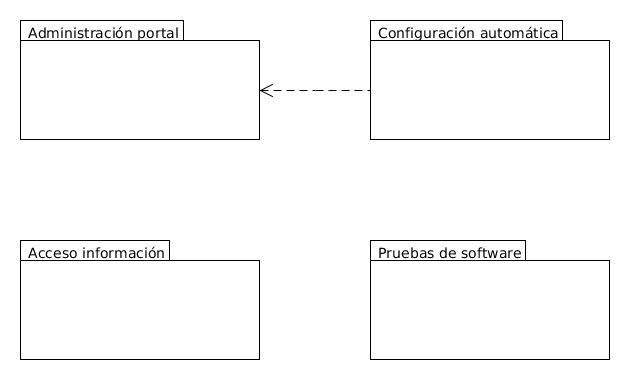
\includegraphics[width=0.8\textwidth]{../images/diagrama_paquetes.png}
  \caption{Diagrama de paquetes}
  \label{fig:diag_paquetes}
  \end{center}
\end{figure}
 
\section{Diagramas de casos de uso}

Los diagramas de casos de uso representa como los diferentes actores se relacionan con el sistema para usar sus funciones. Por ejemplo, en el primer caso de uso vemos como el \textbf{desarrollador} se relaciona con el sistema para iniciar el servidor del portal, mientras, en el segundo vemos como el \textbf{usuario} se relaciona con el sistema para consultar la información de las diferentes secciones del portal.

\begin{figure}[!ht]
  \begin{center}
  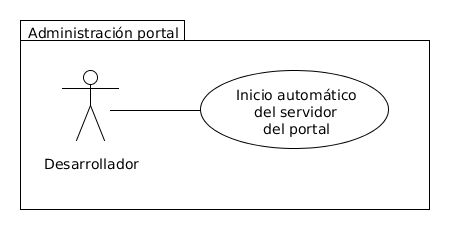
\includegraphics[width=0.65\textwidth]{../images/diag_cu_ap.png}
  \caption{Diagrama de casos de uso: paquete Administración portal}
  \label{fig:diag_cu_ap}
  \end{center}
\end{figure}

\begin{figure}[!ht]
  \begin{center}
  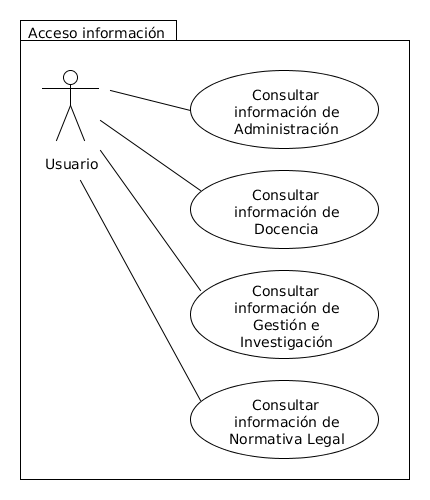
\includegraphics[width=0.65\textwidth]{../images/diag_cu_ai.png}
  \caption{Diagrama de casos de uso: paquete Acceso información}
  \label{fig:diag_cu_ai}
  \end{center}
\end{figure}

\newpage
\
\newpage
En el tercer diagrama vemos como el \textbf{desarrollador} se relaciona con los procesos relacionadas con las pruebas (que a su vez son dependientes entre sí); y en el cuarto vemos como también el \textbf{desarrollador} se relaciona con el sistema para realizar las tareas de configuración automática, como son el despliegue automático y el provisionamiento.

\begin{figure}[!ht]
  \begin{center}
  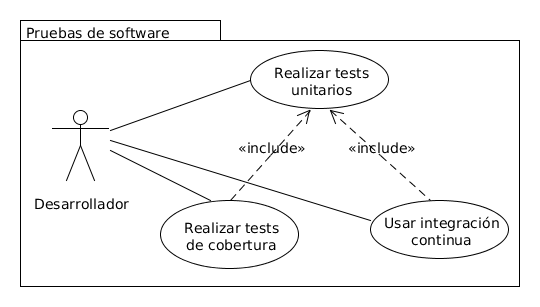
\includegraphics[width=0.65\textwidth]{../images/diag_cu_ps.png}
  \caption{Diagrama de casos de uso: paquete Pruebas de software}
  \label{fig:diag_cu_ps}
  \end{center}
\end{figure}

\begin{figure}[!ht]
  \begin{center}
  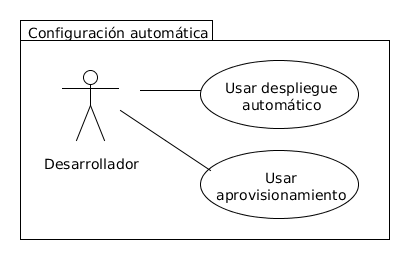
\includegraphics[width=0.65\textwidth]{../images/diag_cu_ca.png}
  \caption{Diagrama de casos de uso: paquete Configuración automática}
  \label{fig:diag_cu_ca}
  \end{center}
\end{figure}

\newpage
\section{Diagramas de actividad}

Los diagramas de actividad sirven para representar la descomposición de un proceso en las diferentes acciones de las que está compuesto. Las actividades de consultar algún tipo de información son procedimiento secuenciales en los que la ejecución es bastante simple; pero la actividad de iniciar el servidor del portal, realizar los test unitarios, realizar los test de cobertura, usar la integración continua tienen situaciones condicionales que son los que dan lugar a cursos alternos de la ejecución. Las actividades de despliegue automático y provisionamiento además tienen también puntos de sincronización que harán que el proceso siga el mismo cauce en su ejecución.

\begin{figure}[!ht]
  \begin{center}
  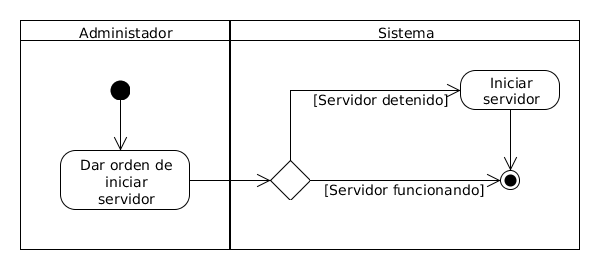
\includegraphics[width=1\textwidth]{../images/diag_act_cu_01.png}
  \caption{Diagrama de actividad CU-1. Inicio automático del servidor del portal}
  \label{fig:diag_act_cu_01}
  \end{center}
\end{figure}

\begin{figure}[!ht]
  \begin{center}
  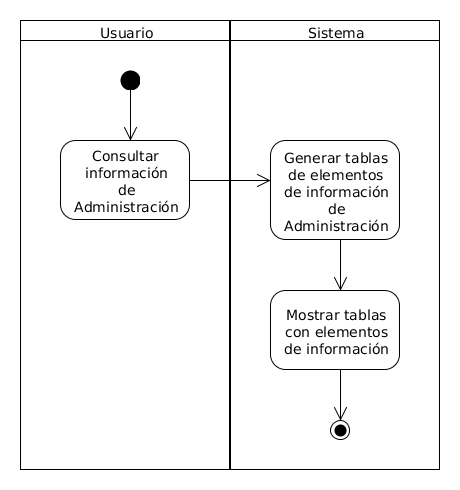
\includegraphics[width=1\textwidth]{../images/diag_act_cu_02.png}
  \caption{Diagrama de actividad CU-2. Consultar información de Administración}
  \label{fig:diag_act_cu_02}
  \end{center}
\end{figure}

\begin{figure}[!ht]
  \begin{center}
  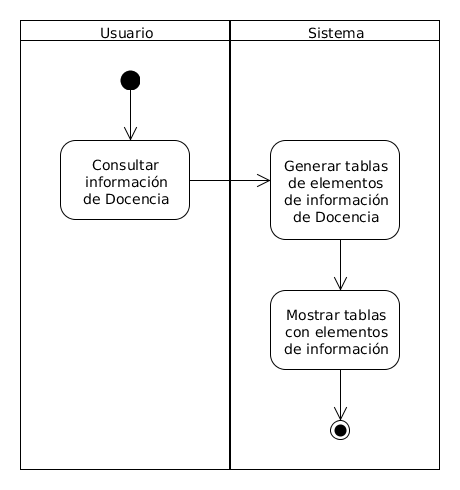
\includegraphics[width=1\textwidth]{../images/diag_act_cu_03.png}
  \caption{Diagrama de actividad CU-3. Consultar información de Docencia}
  \label{fig:diag_act_cu_03}
  \end{center}
\end{figure}

\begin{figure}[!ht]
  \begin{center}
  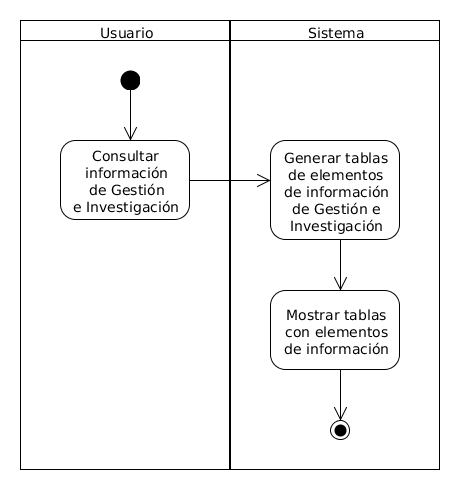
\includegraphics[width=1\textwidth]{../images/diag_act_cu_04.png}
  \caption{Diagrama de actividad CU-4. Consultar información de Gestión e Investigación}
  \label{fig:diag_act_cu_04}
  \end{center}
\end{figure}

\begin{figure}[!ht]
  \begin{center}
  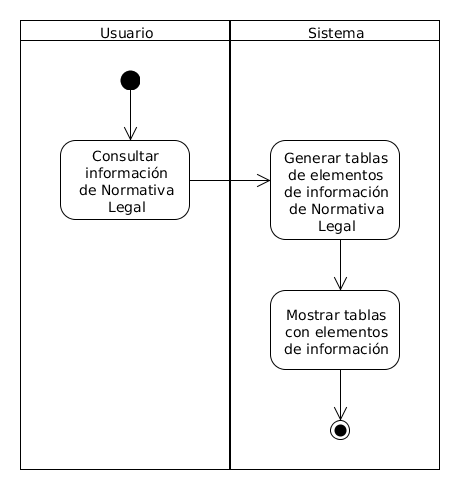
\includegraphics[width=1\textwidth]{../images/diag_act_cu_05.png}
  \caption{Diagrama de actividad CU-5. Consultar información de Normativa Legal}
  \label{fig:diag_act_cu_05}
  \end{center}
\end{figure}

\begin{figure}[!ht]
  \begin{center}
  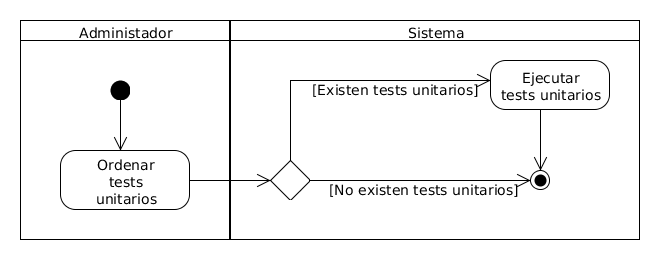
\includegraphics[width=1\textwidth]{../images/diag_act_cu_06.png}
  \caption{Diagrama de actividad CU-6. Realizar tests unitarios}
  \label{fig:diag_act_cu_06}
  \end{center}
\end{figure}

\begin{figure}[!ht]
  \begin{center}
  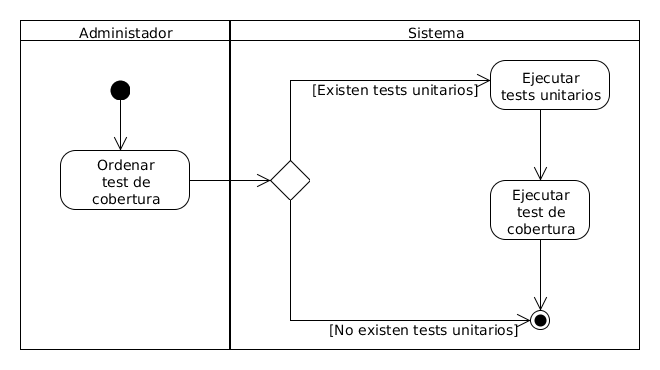
\includegraphics[width=1\textwidth]{../images/diag_act_cu_07.png}
  \caption{Diagrama de actividad CU-7. Realizar test de cobertura}
  \label{fig:diag_act_cu_07}
  \end{center}
\end{figure}

\begin{figure}[!ht]
  \begin{center}
  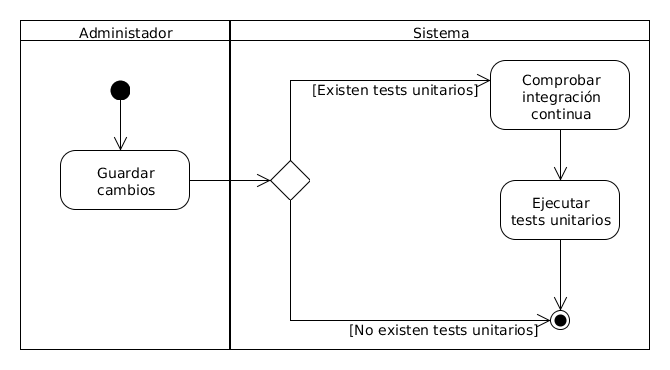
\includegraphics[width=1\textwidth]{../images/diag_act_cu_08.png}
  \caption{Diagrama de actividad CU-8. Usar integración continua}
  \label{fig:diag_act_cu_08}
  \end{center}
\end{figure}

\begin{figure}[!ht]
  \begin{center}
  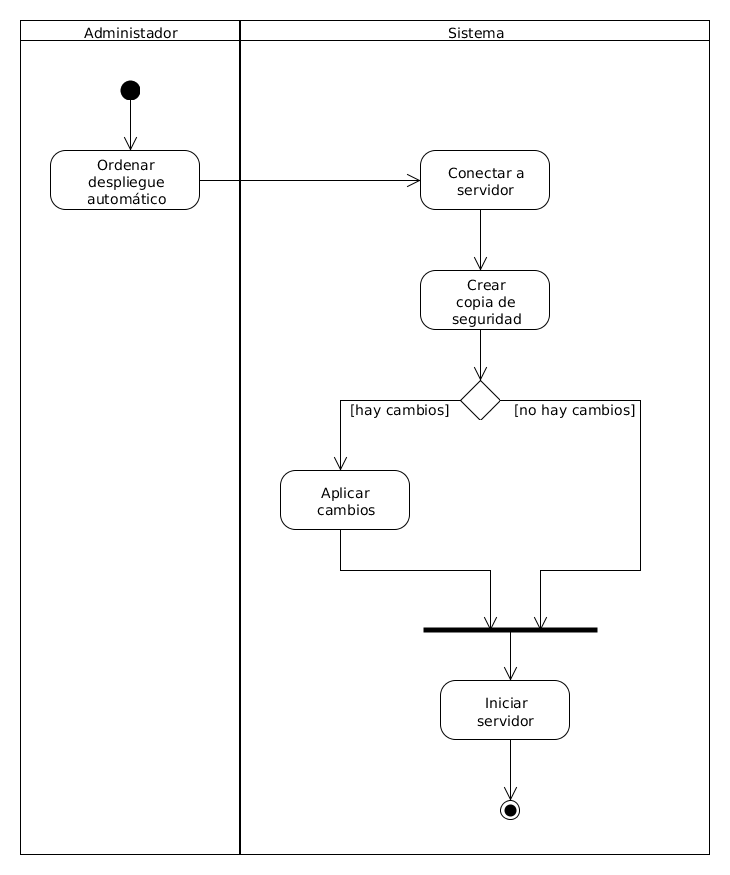
\includegraphics[width=1\textwidth]{../images/diag_act_cu_09.png}
  \caption{Diagrama de actividad CU-9. Usar despliegue automático}
  \label{fig:diag_act_cu_09}
  \end{center}
\end{figure}

\begin{figure}[!ht]
  \begin{center}
  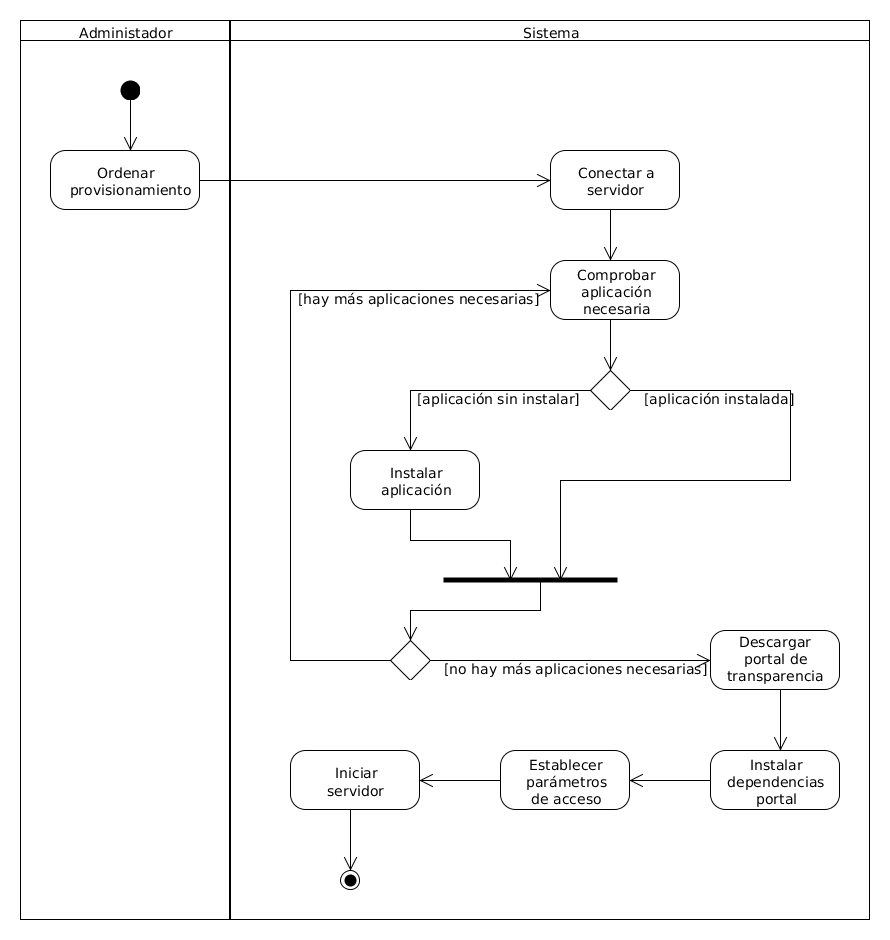
\includegraphics[width=1\textwidth]{../images/diag_act_cu_10.png}
  \caption{Diagrama de actividad CU-10. Usar provisionamiento}
  \label{fig:diag_act_cu_10}
  \end{center}
\end{figure}

\newpage
\
\newpage
\
\newpage
\
\newpage
\
\newpage
\
\newpage
\
\newpage
\
\newpage
\
\newpage

\section{Diagrama conceptual}

En el diagrama conceptual podemos ver una representación de la estructura de la implementación. A excepción de la clase \textbf{test}, todas las clases son parte de la aplicación principal (\textbf{app}) por lo que tienen una relación de composición con la misma y no tienen sentido sin esta. Las clases de \textbf{test} y \textbf{app} tiene una relación de agrupación, porque el módulo test puede realizar las pruebas sobre cualquier módulo de aplicación que sea recibido.

\begin{figure}[!ht]
  \begin{center}
  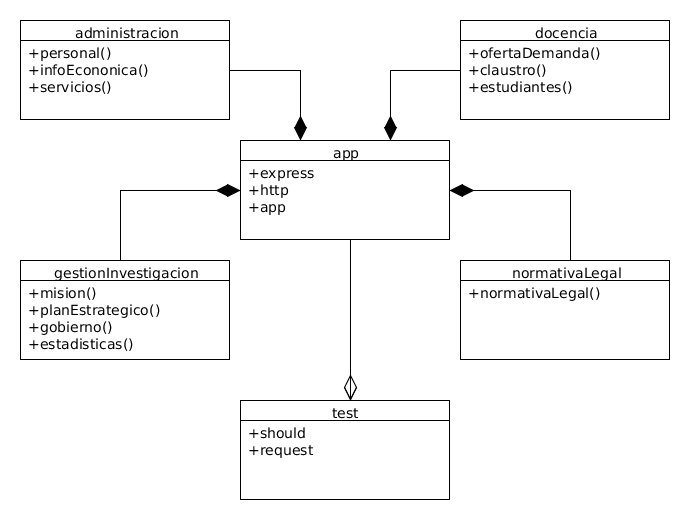
\includegraphics[width=1\textwidth]{../images/diagrama_conceptual.png}
  \caption{Diagrama conceptual}
  \label{fig:diagrama_conceptual}
  \end{center}
\end{figure}

\section{Otros diagramas o interfaces}

Gran parte de la implementación no va a ser de la aplicación principal en si mismo, sino herramientras que se le van a agregar para obtener diferentes funcionalidades que se usarán durante su desarrollo, de ahí que no se considere necesario el realizar diagramas de comunicación ni diagramas de secuencia.

\bigskip
En cuanto a la interfaz gráfica, no será necesaria porque todas las herramientas solo tienen modo de funcionamiento a través de terminal.